\documentclass[a4paper,12pt]{article}
\usepackage{setspace}\setstretch{1.1}
\usepackage[T1]{fontenc}
\usepackage[utf8]{inputenc}
\usepackage{graphicx}
\usepackage{subcaption}
%\usepackage[Conny]{fncychap}
\usepackage{amsmath,amssymb}
\usepackage{fullpage}
\usepackage{subcaption}
\usepackage{ragged2e}
\usepackage{rotating}
\usepackage{multicol}
\usepackage{tabularx}
\usepackage{float}
\usepackage{titlesec}
\usepackage{nicefrac}
\usepackage{titling}
%\numberwithin{figure}{section}
\usepackage{adjustbox}
\usepackage{parskip}
\usepackage{bm,ltablex,microtype}
\usepackage{listings}
\usepackage{xcolor}
\usepackage[final]{pdfpages}
\usepackage[toc,page]{appendix}
\usepackage[margin=0.75in]{geometry}
\usepackage{gensymb}
\usepackage{tgbonum}	      % a font package
\usepackage{booktabs}       % making tables prettier
\renewcommand{\arraystretch}{1.3}


%\color{violet}

\renewcommand{\familydefault}{\sfdefault}

\captionsetup{font=footnotesize, labelfont={bf,sf}}

\raggedbottom

%\def\ga2o3{Ga$_2$O$_3$}
\def\ga2o3{$\beta$-Ga$_2$O$_3$}
\def\cheq{\leftrightharpoons}
\def\deg{$^\circ$C$_{}$}
\date{}
\author{Vilde Mari Reinertsen}

\title{Project 2}

\begin{document}
\begingroup
\let\center\flushleft
\let\endcenter\endflushleft
\maketitle
\endgroup

\begin{abstract}
This is the abstract.
\end{abstract}

\tableofcontents

\section{Introduction}
The main objective of this project is to investigate the many-body problem of simulating a quantum dot. A quantum dot is basically electrons that are trapped in an electrical potential. In this project, the potential is modelled as a harmonic oscillator potential. In this project Variational Monte Carlo (VMC) methods are used to solve the many-body SE for electrons. This project is about the so-called full-shell systems of two, six and twelve electrons in harmonic oscillator traps of different strengths, i.e. trap frequencies. The systems is investigated both for the case where interaction is neglected and included.

The report starts out by introducing the system with the representative equations and analysis tools. Most of the numerical tools used in the programming in this project has already been described in project 1 \cite{project1}, but some additional things are explained or more thoroughly elaborated on in the theory and method part of this report. Furthermore, the results and discussion part first analyses how different important parameters have been chosen, i.e. choice of evaluation of the double derivative, step size of sampling techniques and method and parameters of the optimization. In addition the expectation energies and the one-body densities of the systems involves are compared and evaluated. At last, an evaluation of code's efficiently is made and some concluding remarks are stated.

\section{Theory and method}
In this project we investigate a fermionic system of $N=$ 2, 6 and 12 electrons, where $N$ is the number of particles. It is a so-called closed shell-system. The Hamiltonian used to model this system is

\begin{equation}
\label{eq:finalH}
\hat{H}=\sum_{i=1}^{N} \left(  -\frac{1}{2} \nabla_i^2 + \frac{1}{2} \omega^2r_i^2  \right)+\sum_{i<j}\frac{1}{r_{ij}},
\end{equation}
where 
$$\hat{H}_0=\sum_{i=1}^{N} \left(  -\frac{1}{2} \nabla_i^2 + \frac{1}{2} \omega^2r_i^2  \right)$$
is the single particle part and

\begin{equation}\label{eq:hamilton_interaction}
\hat{H}_1=\sum_{i<j}\frac{1}{r_{ij}},
\end{equation}

represent the interaction potential between particles. The Hamiltonian is written in atomic units, which implies that $\hbar = 1, m= 1$, the unit of length is $a_0 = \nicefrac{4 \pi \epsilon_0 \hbar^2}{m_e e^2}$ and the unit of energy is $E_h = \nicefrac{\hbar^2}{m_e a_0^2}$.  We also have $r_{ij}=\vert \bm{r}_i-\bm{r}_j\vert= \sqrt{(x_i-x_j)^2 + (y_i-y_j)^2}$ and $\omega$ is the oscillator frequency. Later we will study the dependence of the system on the oscillator frequency. 

\subsection{Two particle system}

The single particle wave function in two dimensions is
\begin{equation}\label{eq:single_particle_wf}
\phi_{n_x,n_y}(x,y) = A H_{n_x}(\sqrt{\omega}x)H_{n_y}(\sqrt{\omega}y)\exp{(-\omega(x^2+y^2)/2}.
\end{equation}
where the functions $H_{n_x}(\sqrt{\omega}x)$ are Hermite polynomials,  while $A$ is a normalization constant. The relevant Hermite polynomials in this project are listed in Appendix \ref{app:hermite_and_derivatives}. $\omega$ is the trap frequency.

For the lowest-lying state, $E_{00}$  (see Fig. \ref{fig:states}), we have $n_x=n_y=0$ and an energy $\epsilon_{n_x,n_y}=\omega(n_x+n_y+1) = \omega$, the total energy of the lowest-lying state is hence $2\omega$ because there is room for two electrons with opposite spins. 

\begin{figure}[H]
\center
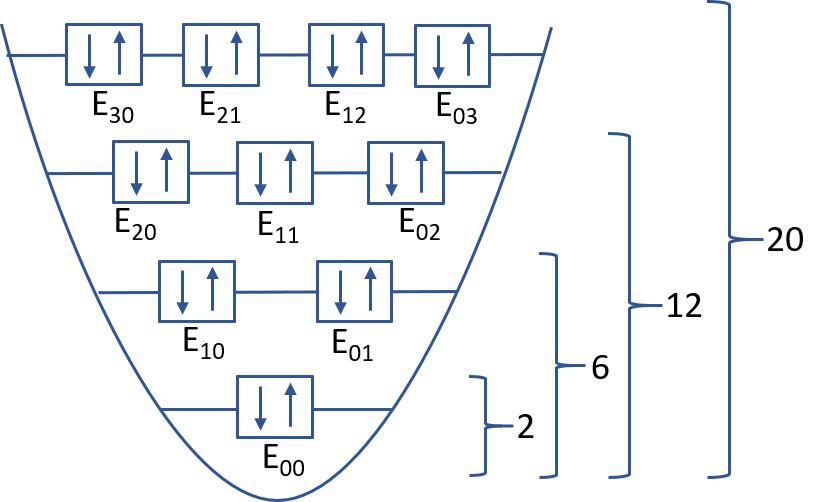
\includegraphics[width=0.6\linewidth]{../Results/states}\caption{Illustration of the different electron states in a harmonic oscillator trap. The numbers $E_{ij}$ represent the different single-particle states and the states at the same level have the same energy. The arrows show that two electrons with opposite spins can occupy the same state. On the right the full shell systems with the according number of particles are pointed out.}\label{fig:states}
\end{figure}

The expectation value can be found by solving the equation

\begin{equation}\label{eq:expectation_energy}
   \langle E \rangle =
   \frac{\int d\bm{r}_1d\bm{r}_2\psi^{\ast}_T(\bm{r}_1,\bm{r}_2)\hat{H}(\bm{r}_1,\bm{r}_2)\psi_T(\bm{r}_1,\bm{r}_2)}
        {\int d\bm{r}_1d\bm{r}_2\psi^{\ast}_T(\bm{r}_1,\bm{r}_2)\psi_T(\bm{r}_1,\bm{r}_2)}.
\end{equation}

We will use Variational Monte Carlo (VMC) methods to evaluate the Eq. \ref{eq:expectation_energy} \cite{project1}. The exact wave function for two not interacting electrons in the ground state is given by

\begin{equation*}
\Phi(\bm{r}_1,\bm{r}_2) = C\exp{\left(-\omega(r_1^2+r_2^2)/2\right)},
\end{equation*}

where $r_i = \sqrt{x_i^2+y_i^2}$ and C is a normalization constant. The trial wavefunction we use for the not interacting case is 
\begin{equation}\label{eq:trial_wf_not_interacing}
\Phi(\bm{r}_1,\bm{r}_2) = C\exp{\left(-\alpha\omega(r_1^2+r_2^2)/2\right)}.
\end{equation}

with the parameter $\alpha$. From the exact wave function we know that $\alpha = 1$ for the situation without interaction. On the other hand, for the interacting case, the trial wave function for the two-electron system is

\begin{equation}
   \psi_{T}(\bm{r}_1,\bm{r}_2) = 
   C\exp{\left(-\alpha\omega(r_1^2+r_2^2)/2\right)}
   \exp{\left(\frac{ar_{12}}{(1+\beta r_{12})}\right)}, 
\label{eq:trial_interacting}
\end{equation}

where we introduce another parameter, $\beta$, and a spin factor, $a$. $a$ is 1 when the two electrons have anti-parallel spins and $1/3$ when they have the parallel spins (this is not relevant before we introduce more particles to the system, as can be seen from Fig. \ref{fig:states}).

\subsection{More particles}

Since we are looking at closed shell systems, the next amount of particles are six. We can see this from Fig. \ref{fig:states}, there are room for two electrons with opposite spin in two different states, in addition to the two in the lowest lying state. The trial wave function is now given by

\begin{equation}
   \psi_{T}(\bm{r}_1,\bm{r}_2,\dots, \bm{r}_6) = 
   Det\left(\phi_{1}(\bm{r}_1),\phi_{2}(\bm{r}_2),
   \dots,\phi_{6}(\bm{r}_6)\right)
   \prod_{i<j}^{6}\exp{\left(\frac{a r_{ij}}{(1+\beta r_{ij})}\right)},
\end{equation}

where 
$$ Det\left(\phi_{1}(\bm{r}_1),\phi_{2}(\bm{r}_2),
   \dots,\phi_{6}(\bm{r}_6)\right) =  \begin{vmatrix}
  \phi_{1}(\bm{r}_1) & \phi_{2}(\bm{r}_1) & \cdots & \phi_{6}(\bm{r}_1) \\
  \phi_{1}(\bm{r}_2) & \phi_{2}(\bm{r}_2) & \cdots & \phi_{6}(\bm{r}_2) \\
  \vdots  & \vdots  & \ddots & \vdots  \\
  \phi_{1}(\bm{r}_6) & \phi_{2}(\bm{r}_6) & \cdots & \phi_{6}(\bm{r}_6) 
\end{vmatrix}$$
is the Slater determinant. This determinant occurs because electron are indistinguishable particles and they are antisymmetric ... . The functions, $\phi_{i}(\bm{r}_j)$,  are given by Eq. \ref{eq:single_particle_wf} and the notation is explained in Tab. \ref{tab:notation_wavefunctions}. 

\begin{table}[H]\caption{The relation between the notation used in the determinant (left) compared to Eq. \ref{eq:single_particle_wf} (right). }\label{tab:notation_wavefunctions}
\large
\center
\begin{tabular}{l|l} 
$\phi_{1}$ & $\phi_{n_x=0, n_y=0}$\\
$\phi_{2}$ & $\phi_{n_x=0, n_y=0}$\\
$\phi_{3}$ & $\phi_{n_x=1, n_y=0}$\\
$\phi_{4}$ & $\phi_{n_x=1, n_y=0}$\\
$\phi_{5}$ & $\phi_{n_x=0, n_y=1}$\\
$\phi_{6}$ & $\phi_{n_x=0, n_y=1}$\\
\end{tabular}
\begin{tabular}{c}
$\,$
\end{tabular}
\begin{tabular}{l|l} 
$\phi_{7}$ & $\phi_{n_x=2, n_y=0}$\\
$\phi_{8}$ & $\phi_{n_x=2, n_y=0}$\\
$\phi_{9}$ & $\phi_{n_x=1, n_y=1}$\\
$\phi_{10}$ & $\phi_{n_x=1, n_y=1}$\\
$\phi_{11}$ & $\phi_{n_x=0, n_y=2}$\\
$\phi_{12}$ & $\phi_{n_x=0, n_y=2}$\\
\end{tabular}
\end{table}

Similarly if we include another "shell" in our system we get 12 particles and the trial wavefunction is 

\begin{equation}
   \psi_{T}(\bm{r}_1,\bm{r}_2, \dots,\bm{r}_{12}) = 
   Det\left(\phi_{1}(\bm{r}_1),\phi_{2}(\bm{r}_2),
   \dots,\phi_{12}(\bm{r}_{12})\right)
   \prod_{i<j}^{12}\exp{\left(\frac{ar_{ij}}{(1+\beta r_{ij})}\right)}.
\end{equation}

The determinant have the same structure as for six particles and the relation to the single-particle wave functions are shown in Tab. \ref{tab:notation_wavefunctions}.

\subsection{One-body density}

The radial one-body density is a measure of the spacial distribution of the electrons with respect to the distance from the middle of the harmonic oscillator trap. To calculate the radial one-body density, we want to sample the position of the electrons. The distance from the origin to a set cut-off is separated into bins with a length $\Delta r$. For every Monte Carlo step, the distance between the electron's position and the origin is calculated, and the bin that corresponds to the current distance get a count. In the end, you have an array corresponding to the different bins with counts corresponding to how many times an electron was found to have that particular distance to the origin. This array is normalized by dividing by the number of Monte Carlo steps. However, to get the density, we have to divide the number in the bins with the area or volume the bin represents. Because we have two-dimensional problem in this project and we calculate the radial one-body density, we divide bin $i$ with the area $ A = \pi (r_i+\Delta r)^2 - \pi r_i^2$ where $r_i$ is distance from the origin to bin $i$. \textit{normalized to the number of particles. Mention. Should happen automatically... Does not happen automatically for me, but I have notice that Even has the same scale on the y-axis.}\cite{Evens_master}

\subsection{Virial theorem}

The virial theorem gives a relation between the time-average total kinetic energy, $\left<T\right>$, and the time-average external potential energy, $\left<V_{ext}\right>$, that is

\begin{equation}\label{eq:virial_theorem}
2\left< T\right> = n\left< V_{ext}\right>
\end{equation}

where $V(r) = Br^n$. In our case when we do not include interaction $n = 2$ from the external potential term in Eq. \ref{eq:finalH}, and therefore the average kinetic energy should be equal to the average potential energy. This can be used as a test to see if the simulations executed are correct. 

\subsection{Trap frequency}

The trap frequency changes the external potential felt by the electrons. Figure \ref{fig:harmonic_oscillator_potential} shows how a larger trap frequency, $\omega$, results in a narrower external potential. In this narrow harmonic oscillator trap, the electrons are forced to be closer to each other. Later, we will investigate how $\omega$ affects the energy when the electrons are interacting with each other through the potential given in Eq. \ref{eq:hamilton_interaction}

\begin{figure}[H]
\center
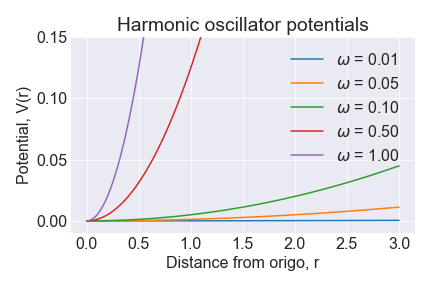
\includegraphics[width=0.7\linewidth]{../Results/harmonic_oscialltor_potentials}\caption{Illustration of how the potential changes when the trap frequency changes. }\label{fig:harmonic_oscillator_potential}
\end{figure}

\subsection{Evaluating the error}

Standard error of the mean (SEM):
\begin{equation}
\text{SEM} = \frac{\sigma}{\sqrt{N}}
\end{equation}
where $N$ is the number of observations, in our case the number of Monte Carlo cycles.

\subsection{The program}

\textit{A short introduction?}

\subsubsection{Initialization}

First the different parts of the program is initialized based on what Hamiltonian that is used and what wave function is used. In this program, one can choose an Hamiltonian with and without interaction (InteractionHarmonicOscillator and HarmonicOscillator, respectively), and accordingly a wave function with and without a Jastrow factor (SlaterDeterminantInteraction and Slaterdeterminant, respectively). Thereafter, the initial state is set up. The particles are distributed after randomly after a set distribution. Two different distributions are used and chosen based on the sampling method. For importance sampling a Gaussian distrribution is used (GaussainDistribution) and for brute force sampling a random uniform distribution is used (RandomUniform). This initialization reflects in the way the sampling of new positions are made by the sampling method, which is explained in project 1 \cite{project1}.

\subsubsection{Metropolis steps}

After the initialization the particles are moved one by one, chosen at random, and the new position is found through the sampling method. The metropolis ratio is calculated to determine wether the step is accepted or not. The metropolis ratio is also determined by the sampling method. If the step is accepted, the energy is sampled and if not, the former energy is sampled again. This is continued until all Monte Carlo (MC) cycles have finished. 

\subsubsection{Sampling}

In this program one can choose to sample all local energies for all MC cycles. This makes it possible to performed resampling techniques on the dataset to improve estimate of the error by estimating the correlation between the different metropolis steps, i.e. the samples made of the local energy. For the other outputs, e.g. kinetic, potential and interaction energy and the mean distance, the average is calculated based on the sum of all the sampled values by dividing by the number of MC cycles.

\subsection{Improving performance and effiency}

\subsubsection{Vectorization}

Solving as vectors instead of scalars - using more of memory - is sort of parallel. 

\subsubsection{Parallelizing}

Doing operations in parallell instead of secquentially. In this case, we want more MC cycles in less time. I chose to parallellize with cmake. I am generating files that contain $E_L$. I get the same data if I run the same code (with different seeds for the random number generator) in 4 proseccors for MC cycles/4 or the same code for MC cycles in one proscessor. Embarrasing parallellization - very simple. Need different file name. 

\subsubsection{Reducing computational cost}

Decrease floating point operations (flops) by smarter code and use of ratios.

\section{Results and discussion}
\subsection{Two electrons in two dimensions}

We start with the simple case of two electrons in a harmonic oscillator trap. These electrons do not interact with eachother and the trial wavefunction is given by Eq. \ref{eq:trial_wf_not_interacing}. 

\subsubsection{Brute force sampling}

First, brute force sampling was used to calculate the new position and evaluate the metropolis ratio. The double derivative of the wavefunction, used to calculate the kinetic energy part of the expectation energy, was evaluated both analytically and numerically. Table \ref{tab:brute_force_no_interaction_2p} shows the energy for different values for the parameter $\alpha$. The numbers show that the standard error of the mean (SEM) is underestimating the deviations. From Tab. \ref{tab:brute_force_no_interaction_2p} one can observe that including the correlations, e.g. correlations in the random number generator, increases the deviation, giving us $\sigma_b$. This value is also an estimate of the error, but probably a more true estimate of the error.

From Tab. \ref{tab:brute_force_no_interaction_2p} one can also observe that $\alpha $ = 1.0 gives zero standard deviation and is therefore the optimal parameter. By comparing the results for the analytical and the numerical cases one can observe that the SEM and $\sigma_b$ is similar for both cases, especially around the ground state ($\alpha$ = 1.0). If he expectation energies from the analytial case and the numbercal cases are compared, they differ with values at the scale of $10^{-3}$, which is reasonable with a $\sigma_b$ around $10^{-3}$ to $10^{-2}$. At last one can observe, both from the individual CPU time measurements and the mean CPU time of these 10 measurements (though with different $\alpha$s), that the analytical solution of the double derivative is much faster and more efficient than the numerical case. 

\begin{table}[H]\caption{Comparing the results for analytical/numerical evaluation of the double derivative. Energy are in atomic units (a.u.) and CPU time is in units of seconds. Number of MC cycles are 2$^{21}$.}\label{tab:brute_force_no_interaction_2p}
\center
\begin{tabular}{l|l}
Analytical: &  Numerical:\\ \hline
\begin{tabular}{ccccc}
$\alpha$: & $\left< E_L \right>$: & SEM: & $\sigma_B$: & CPU time:\\ \hline
0.50 & 2.49402 & 0.00073 & 0.01022 & 5.57812\\
0.60 & 2.26441 & 0.00052 & 0.00690 & 5.76562\\
0.70 & 2.13118 & 0.00035 & 0.00448 & 5.92188\\
0.80 & 2.05016 & 0.00022 & 0.00263 & 5.67188\\
0.90 & 2.01015 & 0.00010 & 0.00116 & 5.96875\\
1.00 & 2.00000 & 0.00000 & 0.00000 & 5.62500\\
1.10 & 2.00871 & 0.00009 & 0.00102 & 6.20312\\
1.20 & 2.03402 & 0.00018 & 0.00175 & 6.34375\\
1.30 & 2.07259 & 0.00026 & 0.00244 & 5.95312\\
1.40 & 2.11041 & 0.00034 & 0.00311 & 6.15625\\ \hline
\end{tabular} & \begin{tabular}{ccccc}
$\alpha$: & $\left< E_L \right>$: & SEM: & $\sigma_B$: & CPU time:\\ \hline
0.50 & 2.49991 & 0.00073 & 0.01093 & 18.20310\\
0.60 & 2.26412 & 0.00053 & 0.00727 & 18.21880\\
0.70 & 2.13039 & 0.00036 & 0.00436 & 18.62500\\
0.80 & 2.04993 & 0.00022 & 0.00269 & 18.46880\\
0.90 & 2.01160 & 0.00010 & 0.00118 & 18.46880\\
1.00 & 2.00000 & 0.00000 & 0.00000 & 18.31250\\
1.10 & 2.00825 & 0.00009 & 0.00097 & 18.35940\\
1.20 & 2.03308 & 0.00018 & 0.00170 & 18.31250\\
1.30 & 2.06460 & 0.00026 & 0.00243 & 20.23440\\
1.40 & 2.11803 & 0.00033 & 0.00308 & 19.00000\\ \hline
\end{tabular}\\
Mean CPU time: 5.91875 & Mean CPU time:  18.62033\\
\end{tabular}
\end{table}

\subsubsection{Including importance sampling}

Figure \ref{fig:comparing_sampling} compare the expectation value of the energy and the acceptance rate of brute force sampling and importance sampling. It can be observed from the right part of the figure that the acceptance rate of both methods increase with decreasing step size, but one can also observe that the acceptance is lower for importance sampling than brute force sampling at large step sizes. These observations could indicate that a small step size would be ideal for both methods. 

\begin{figure}[H]
\center
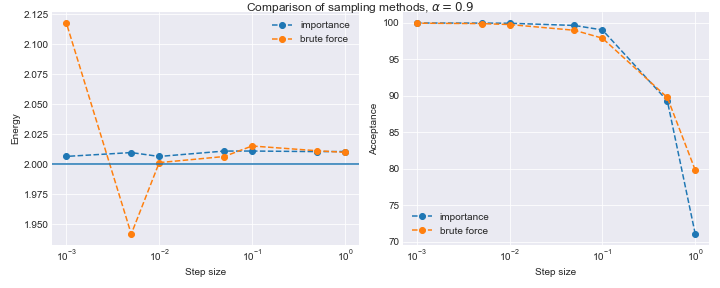
\includegraphics[width=\linewidth]{../Results/comparing_sampling}\caption{Left: Expectation energies after $2^{21}$ MC cycles for different step sizes. Right: Percentage of accepted steps for different step sizes. Here importance sampling and brute force sampling is compared. }\label{fig:comparing_sampling}
\end{figure}


From the left part of the figure it can be observed that one of the expectation values for the energies are lower than the ground state energy ($dl = 0.005$ with brute force sampling) when these calculations where done with $\alpha$ = 0.9. However, in Tab. \ref{tab:importance_no_interaction_2p} which compare the result of brute force sampling and importance sampling for different step sizes one can observe that the standard deviation from the blocking method is larger for the case of brute force sampling with a step size of 0.005. However,  the SEM does not indicate anything to be special about this result.

\begin{table}[H]\caption{Comparing the results for importance/brute force sampling. Energy are in atomic units (a.u.) and CPU time is in units of seconds. Here the parameter $\alpha$ is set to 0.9 and number of MC cycles are 2$^{21}$.}\label{tab:importance_no_interaction_2p}
\begin{tabular}{l|l|l} 
 & Brute force: &  Importance:\\ \hline
\begin{tabular}{c} 
$dl$:\\ \hline
1.000\\
0.500\\
0.100\\
0.050\\
0.010\\
0.005\\
0.001\\
\end{tabular} & \begin{tabular}{ccccc}
 $\left< E_L \right>$: & SEM: & $\sigma_B$: & Acc.: & $t_{CPU}$:\\ \hline
2.010 & 0.00010 & 0.00066 & 79.832& 6.625\\
2.011 & 0.00010 & 0.00112 & 89.794& 7.266\\
2.015 & 0.00011 & 0.00549 & 97.919& 7.078\\
2.007 & 0.00011 & 0.00946 & 99.001& 7.016\\
2.002 & 0.00007 & 0.01510 & 99.788& 6.953\\
1.942 & 0.00006 & 0.02140 & 99.916& 6.578\\
2.118 & 0.00002 & 0.00371 & 99.974& 6.531\\ \hline
\end{tabular} & \begin{tabular}{ccccc}
$\left< E_L \right>$: & SEM: & $\sigma_B$: & Acc.: & $t_{CPU}$:\\ \hline
2.011 & 0.00010 & 0.00022 & 71.078& 8.531\\
2.011 & 0.00010 & 0.00023 & 89.343& 8.672\\
2.011 & 0.00010 & 0.00047 & 99.049& 8.859\\
2.011 & 0.00010 & 0.00068 & 99.662& 8.188\\
2.007 & 0.00010 & 0.00136 & 99.968& 8.281\\
2.010 & 0.00010 & 0.00199 & 99.989& 8.547\\
2.007 & 0.00010 & 0.00410 & 99.999& 8.016\\ \hline
\end{tabular}\\
& Mean CPU time: 6.86384 & Mean CPU time: 8.44197 \\
\end{tabular}
\end{table}

I took a closer look at the actual local energies for the brute force sampling method. Figure \ref{fig:brute_force_small_steps} shows how the energy is not stable for steps sizes smaller than 0.01, so even though the step sizes 0.001 and 0.01 seems to give reasonable expectation values for the energy (see Tab. \ref{tab:importance_no_interaction_2p} and Fig. \ref{fig:comparing_sampling}), Fig. \ref{fig:brute_force_small_steps} seems to show that that is sort of a lucky shot. I also saw this by running the calculation with brute force sampling and the step size, $0.005$, with different seeds for the random number generator. The expectation energy for five different runs where $\left< E_L \right>$ =  1.91487, 2.03452, 1.90805, 1.88356 and 1.9284. From Fig. \ref{fig:brute_force_larger_steps} one can observe that even $dl=0.1$ seems to be too small since it also results in the local energy varying slowly and taking longer "trips" to higher energies and using many steps to get back down again, but for this step size the "trips" to higher energies are more frequent than for the smaller step sizes. I concluded that a step size of 0.5 is the best choice for the brute force sampling because it gives resonable changes of the local energy and an accpentance rate of $\sim$ 90 \% (see Fig. \ref{fig:comparing_sampling}). 

\begin{figure}[H]
\begin{subfigure}{.5\textwidth}
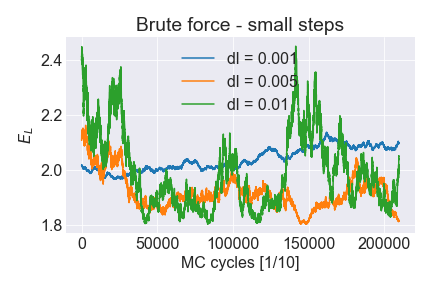
\includegraphics[width=\linewidth]{../Results/brute_force_small_steps}\caption{}\label{fig:brute_force_small_steps}
\end{subfigure}
\begin{subfigure}{.5\textwidth}
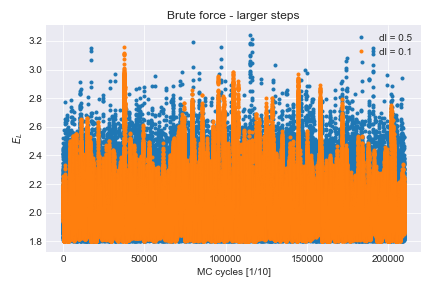
\includegraphics[width=\linewidth]{../Results/brute_force_larger_steps}\caption{}\label{fig:brute_force_larger_steps}
\end{subfigure}
\caption{The local energy for every tenth MC cycle for brute force sampling at different step sizes, $dl$. a) shows the smaller step sizes and b) some that are a bit larger. }\label{fig:brute_force_step_sizes}
\end{figure}

%On the other hand, for the importance sampling, the investigation of the local energies did not give any clues to why the expecation energy is lower that the ground state energy for a step size of 0.5. Eventually I decided that the result itself indicate that 0.5 is a too large step size for importance sampling and taken together with a low acceptance rate at 0.5 ($\sim$ 82 \%) it is clear that a smaller step size is preferable. 
%
%At last, it is interesting to note that the CPU time of importance sampling is higher than the brute force sampling, so even though brute force sampling has a lower acceptance rate, at the ideal step size, than importance sampling the two methods seems to be somewhat comparable at least for the system I am investigating.

Proceeding to evaluate the energy, Table \ref{tab:ground_state_energy_different_omegas_no_interaction_2p} shows how the energy changes with different trap frequencies, $\omega$. In this table one can observe that there is no large difference between the reuslts from brute force sampling and importance sampling. However, to be able to compare the sampling methods more thoroughly it is better to look at the case where the system is not in the ground state. 

\textit{JEG KOM HIT :)}

\begin{table}[H]\caption{Ground state energy of two electrons in harmonic oscillator trap. Number of MC cycles are $2^{23}$.}\label{tab:ground_state_energy_different_omegas_no_interaction_2p}
\begin{tabular}{l|l|l} 
 & Brute force: &  Importance:\\ \hline
\begin{tabular}{c} 
$\omega$  \\ \hline
1.00  \\
0.50  \\
0.10  \\
0.05  \\
0.01  \\
\end{tabular} & \begin{tabular}{ccccc}
$\alpha$ & $\left< E_L \right>$ & $\overline{r}_{12} $ & $\left< T \right>$  & $\left< V_{ext}\right>$ \\ \hline
1 & 2.00 & 1.250 & 1.0008 & 0.9992\\
1 & 1.00 & 1.775 & 0.4971 & 0.5029\\
1 & 0.20 & 3.967 & 0.0996 & 0.1004\\ 
1 & 0.10 & 5.638 & 0.0497 & 0.0503\\ 
1 & 0.02 & 12.631 & 0.0099 & 0.0101\\  
\end{tabular} & \begin{tabular}{ccccc}
$\alpha$ & $\left< E_L \right>$ & $\overline{r}_{12} $ & $\left< T \right>$  & $\left< V_{ext}\right>$ \\ \hline
1 & 2.00 & 1.254 & 0.9982 & 1.0018\\
1 & 1.00 & 1.781 & 0.4973 & 0.5027\\
1 & 0.20 & 4.046 & 0.0987 & 0.1013\\ 
1 & 0.10 & 5.534 & 0.0512 & 0.0488\\ 
1 & 0.02 & 12.488 & 0.0101 & 0.0099\\ 
\end{tabular}\\
\end{tabular}
\end{table}

\begin{table}[H]\caption{Comparing the results for brute force sampling/importance sampling. Energy are in atomic units (a.u.) and CPU time is in units of seconds. Number of MC cycles are 2$^{21}$.}\label{tab:compare_importance_alphas_2p}
\center
\begin{tabular}{l|l|l}
 & Brute force: & Importance:\\ \hline
\begin{tabular}{c}
$\alpha$: \\ \hline
0.50 \\
0.60 \\
0.70 \\
0.80 \\
0.90\\
1.00 \\
1.10 \\
1.20 \\
1.30\\
1.40 \\ \hline
\end{tabular} & \begin{tabular}{cccc}
 $\left< E_L \right>$: & SEM: & $\sigma_B$: & CPU time:\\ \hline
2.49074 & 0.00072 & 0.01030 & 6.26562\\
2.27645 & 0.00053 & 0.00721 & 6.53125\\
2.12481 & 0.00036 & 0.00451 & 6.59375\\
2.04873 & 0.00022 & 0.00265 & 6.68750\\
2.01135 & 0.00010 & 0.00115 & 6.82812\\
2.00000 & 0.00000 & 0.00000 & 6.75000\\
2.00863 & 0.00009 & 0.00097 & 6.59375\\
2.03343 & 0.00018 & 0.00174 & 7.29688\\
2.07103 & 0.00026 & 0.00246 & 6.75000\\
2.11725 & 0.00033 & 0.00317 & 6.70312\\ \hline
\end{tabular} & \begin{tabular}{cccc}
$\left< E_L \right>$: & SEM: & $\sigma_B$: & CPU time:\\ \hline
2.52950 & 0.00075 & 0.01952 & 8.53125\\
2.26531 & 0.00052 & 0.01281 & 8.62500\\
2.12449 & 0.00036 & 0.00813 & 8.76562\\
2.04797 & 0.00022 & 0.00454 & 9.37500\\
2.01171 & 0.00010 & 0.00203 & 8.81250\\
2.00000 & 0.00000 & 0.00000 & 8.76562\\
2.00954 & 0.00009 & 0.00171 & 8.40625\\
2.03276 & 0.00018 & 0.00305 & 8.50000\\
2.07363 & 0.00026 & 0.00440 & 8.67188\\
2.10697 & 0.00034 & 0.00536 & 8.67188\\ \hline
\end{tabular}\\
& Mean CPU time:  6.7000 & Mean CPU time:  8.7125\\
\end{tabular}
\end{table}

\subsubsection{Including optimization}

Minimization rate of 0.5 seemed to be ideal. It resulted in the fewest steps until the parameter value stabilized both for guesses close to the optimal value and for guesses far away from the optimal value, but for the smallest trap frequencies I had to use $\gamma = $ 0.1 or 0.2. The parameters were optimized by trying out different first guesses for $\alpha$ and $\beta$ and tuning $\gamma$ so that the parameters stabilized during the first 200 iteretions. The optimal parameters were extracted from the mean of the last 50 iterations. An example run is shown in Fig. \ref{} for $\omega = 0.5$.

\subsubsection{Including interaction}

\begin{table}[H]\caption{Ground state energy of two interacting electrons in harmonic oscillator trap found with brute force sampling. Number of MC cycles are $2^{23}$}\label{tab:ground_state_energy_brute_force_interaction}
\center
\begin{tabular}{c|cccccrccc}
$\omega$ & $\alpha$ & $\beta$ & $\left< E_L \right>$ & SEM & $\sigma_B$ &  $\overline{r}_{12} \,\,\,$ & $\left< T \right>$  & $\left< V_{ext}\right>$ & $\left<V_{int} \right>$  \\ \hline
1.00 & 0.98847 & 0.39965 & 3.0068 & 0.00001 & 0.00009 & 1.636 & 0.8944 & 1.2990 & 0.8135\\
0.50 & 0.98061 & 0.31091 & 1.6674 & 0.00001 & 0.00010 & 2.481 & 0.4488 & 0.7051 & 0.5135\\
0.10 & 0.94693 & 0.17764 & 0.4486 & 0.00001 & 0.00011 & 6.695 & 0.1003 & 0.1767 & 0.1716\\
0.05 & 0.92747 & 0.13815 & 0.2609 & 0.00000 & 0.00011 & 10.389 & 0.0533 & 0.0997 & 0.1076\\
0.01 & 0.88398 & 0.07287 & 0.0777 & 0.00000 & 0.00006 & 29.177 & 0.0129 & 0.0284 & 0.0364\\
\end{tabular}
\end{table}

\begin{table}[H]\caption{Ground state energy of two interacting electrons in harmonic oscillator trap found with importance sampling. Number of MC cycles are $2^{23}$}\label{tab:ground_state_energy_importance_interaction}
\center
\begin{tabular}{c|ccccccccc}
$\omega$ & $\alpha$ & $\beta$ & $\left< E_L \right>$ & SEM & $\sigma_B$ &  $\overline{r}_{12} \,\,\,$ & $\left< T \right>$  & $\left< V_{ext}\right>$ & $\left<V_{int} \right>$  \\ \hline
1.00 & 0.98846 & 0.39954 & 3.0069 & 0.00001 & 0.00018 & 1.643 & 0.8931 & 1.3052 & 0.8086\\
0.50& 0.98082 & 0.31068 & 1.6674 & 0.00001 & 0.00019 & 2.481 & 0.4547 & 0.6997 & 0.5130\\
0.10 & 0.94734 & 0.17810 & 0.4486 & 0.00001 & 0.00023 & 6.724 & 0.0989 & 0.1787 & 0.1710\\
0.05 & 0.92262 & 0.14090 & 0.2610 & 0.00000 & 0.00021 & 10.333 & 0.0495 & 0.1024 & 0.1091\\
\end{tabular}
\end{table}

\subsection{One-body density}

\begin{figure}[H]
\center
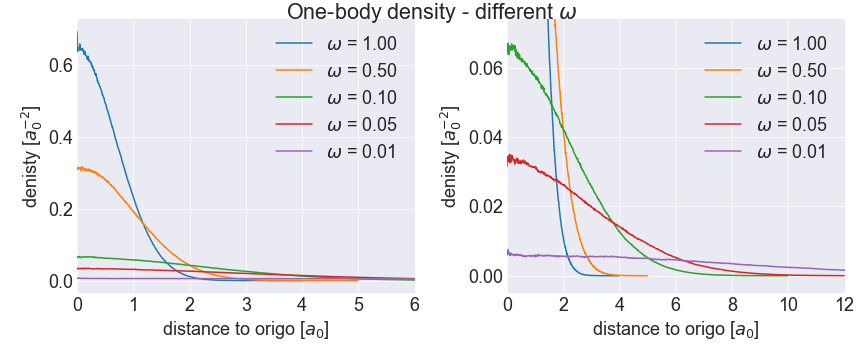
\includegraphics[width=0.8\linewidth]{../Results/one_body_density_no_interaction_2p}\caption{•}\label{fig:one_body_density_no_interaction_2p}
\end{figure}

\begin{figure}[H]
\center
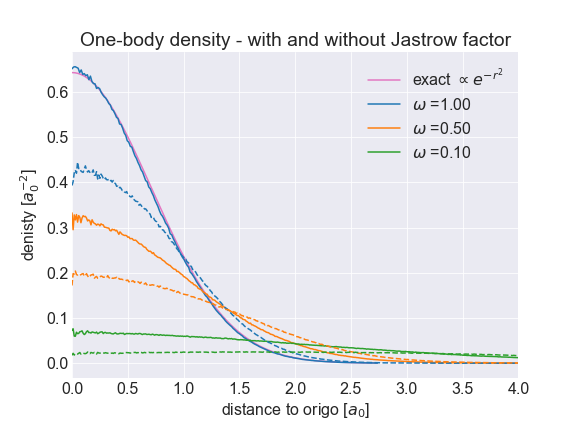
\includegraphics[width=0.7\linewidth]{../Results/one_body_density_interaction_2p}\caption{Dashed lines are with the Jastrow factor. Normal lines is without Jastrow factor. }\label{fig:one_body_density_interaction_2p}
\end{figure}

\subsection{Extending to more particles}

\subsubsection{Six particles}

\begin{table}[H]\caption{Number of MC cycles are $2^{23}$. }\label{tab:ground_state_energy_importance_6p}
\center
\begin{tabular}{c|rcc}
$\omega$ & $\left< E_L \right>$  & $\left< T \right>$  & $\left< V_{ext}\right>$ \\ \hline
1.00 & 10.00 & 4.9865 & 5.0135\\ 
0.50 & 5.00 & 2.4973 & 2.5027\\
0.10 & 1.00 & 0.4861 & 0.5139\\
0.05 & 0.50 & 0.2483 & 0.2517\\
0.01 & 0.10 & 0.0454 & 0.0546\\
\end{tabular}
\end{table}

\begin{table}[H]\caption{Ground state energy of two interacting electrons in harmonic oscillator trap found with importance sampling. Number of MC cycles are $2^{23}$}\label{tab:ground_state_energy_importance_interaction_6p}
\center
\begin{tabular}{c|cccccccc}
$\omega$ & $\alpha$ & $\beta$ & $\left< E_L \right>$ & SEM & $\sigma_B$ &  $\left< T \right>$  & $\left< V_{ext}\right>$ & $\left<V_{int} \right>$  \\ \hline
1.00 & 0.71567 & 0.49372 & 20.4492 & 0.00022 & 0.00813 & 2.3429 & 10.7076 & 7.3988\\
0.50 & 0.75823 & 0.34260 & 11.9868 & 0.00011 & 0.00522 & 1.3226 & 5.8094 & 4.8548\\
0.10 & 0.78852 & 0.15041 & 3.6542 & 0.00003 & 0.00416 & 0.2951 & 1.7035 & 1.6556\\
0.05 & 0.76518 & 0.10733 & 2.2223 & 0.00003 & 0.00436 &  0.1178 & 1.0882 & 1.0162\\
\end{tabular}
\end{table}

\begin{figure}[H]
\center
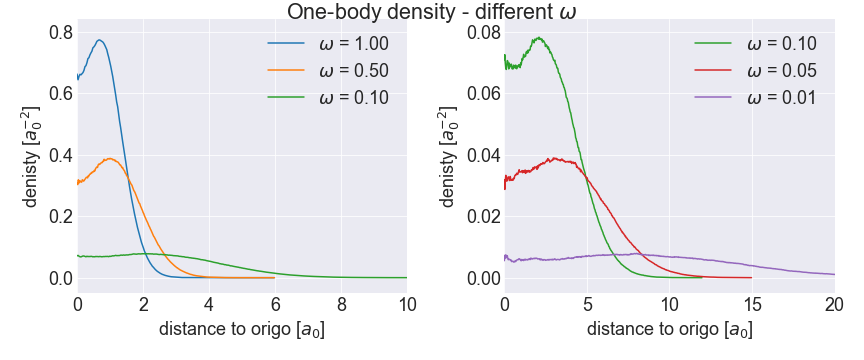
\includegraphics[width=0.8\linewidth]{../Results/one_body_density_no_interaction_6p}\caption{•}\label{fig:one_body_density_no_interaction_6p}
\end{figure}

\begin{figure}[H]
\center
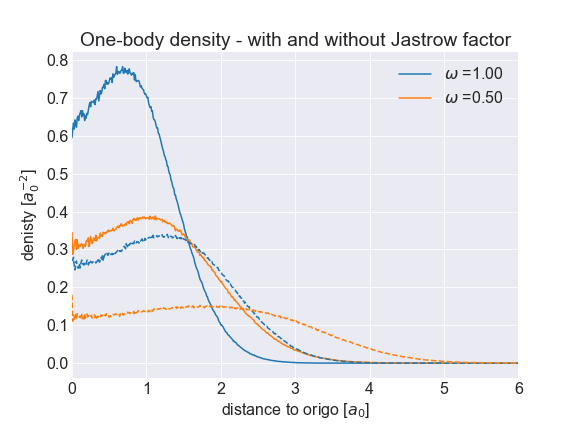
\includegraphics[width=0.7\linewidth]{../Results/one_body_density_interaction_6p}\caption{Dashed lines are with the Jastrow factor. Normal lines is without Jastrow factor. }\label{fig:one_body_density_interaction_6p}
\end{figure}


\subsubsection{Twelve particles}

\begin{table}[H]\caption{Number of MC cycles are $2^{23}$. }\label{tab:ground_state_energy_importance_12p}
\center
\begin{tabular}{c|rrr}
$\omega$ & $\left< E_L \right>$  & $\left< T \right>\,\,\,$  & $\left< V_{ext}\right>\,$ \\ \hline
1.00 & 28.00 & 14.0117 & 13.9883\\ 
0.50 & 14.00 & 7.0463 & 6.9537\\ 
0.10 & 2.80 & 1.4084 & 1.3916\\ 
0.05 & 1.40 & 0.6901 & 0.7099\\ 
0.01 & 0.28 & 0.1419 & 0.1381\\ 
\end{tabular}
\end{table}

\begin{figure}[H]
\center
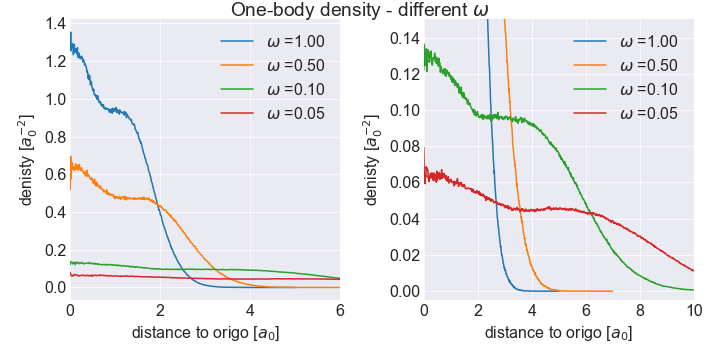
\includegraphics[width=0.8\linewidth]{../Results/one_body_density_no_interaction_12p}\caption{Had to use MC 2 24 to get smooth graphs. }\label{fig:one_body_density_no_interaction_12p}
\end{figure}

\begin{appendices}
\section{Dealing with the Slater determinant efficiently}

In the metropolis test we calculate the ratio bewteen the wavefunction before and after a proposed move, but now the wavefunction includes a determinant which is costly to calculate. We therefore want to utilize some relations from linear algebra to simplify the ratio and make the algorithm more efficent. The ratio between the Slater determinant part of the wavefunction, $\psi_{SD}$, is
\begin{equation}\label{eq:metropolis_ratio}
R = \frac{\psi_{SD}(\bm{r}^{new})}{\psi_{SD}(\bm{r}^{old})} = \frac{\sum_i^N d_{ij}(\bm{r}^{new})C_{ij}(\bm{r}^{new})}{\sum_i^N d_{ij}(\bm{r}^{old})C_{ij}(\bm{r}^{old})}.
\end{equation} where $d_{ij} = \psi_i(j)$

Here we have used the fact that when you calculate a determinant, you break it down into a sum of smaller determinants times a factor:

\begin{equation*}
D = 
 \begin{vmatrix}
  d_{11} & d_{12} & \cdots & d_{1N} \\
  d_{21} & d_{22} & \cdots & d_{2N} \\
  \vdots  & \vdots  & \ddots & \vdots  \\
  d_{N1} & d_{N2} & \cdots & d_{NN} 
\end{vmatrix} = \sum_i^N d_{ij}C_{ij}. %= \sum_i^Nd_{ij}(-1)^{i+j}M_{ij}.
\end{equation*}

So if $d{ij} = d_{11}$ then 
\begin{equation*}
C_{11} = 
 \begin{vmatrix}
 d_{22} & d_{23} & \cdots & d_{2N} \\
  d_{32} & d_{33} & \cdots & d_{3N} \\
  \vdots  & \vdots  & \ddots & \vdots  \\
  d_{N2} & d_{N3} & \cdots & d_{NN} 
 \end{vmatrix}.
\end{equation*}

%This matrix can also be expressed using what is called minors. The minor, $M_{23}$, of a matrix, $M$ is the determinant of the matrix $M$, where row 2 and coloumn 3 is removed. The determinant $C$ from above can be expressed in minors as
%$ C_{ij} = (-1)^{j+i}M_{ij}$ where the factor $(-1)^{j+i}$ ensures the correct sign.

We observe in Eq. \ref{eq:metropolis_ratio} that if we move particle $j$ from $r_j^{old}$ to $r_j^{new}$ the matrix $C_{ij}$ is unchanged, we have only changed the $d_{ij}$ in the original determinant $D$ that is not included in $C_{ij}$. Equation \ref{eq:metropolis_ratio} is then

\begin{equation}
R = \frac{\sum_i^N d_{ij}(\bm{r}^{new})}{\sum_i^N d_{ij}(\bm{r}^{old})}
\end{equation}

We can simplify this even further with the relation

\begin{equation}
\sum_{k=1}^N d_{ik}^{}d_{kj}^{-1} = \delta_{ij} = \left\{ \begin{matrix}
0 \quad \text{ if } i \neq j \\
1 \quad \text{ if } i = j
\end{matrix} \right. 
\end{equation}

The ratio can be rewritten as

\begin{equation}
R = \frac{\sum_i^N d_{ij}(\bm{r}^{new})d_{ij}(\bm{r}^{old})^{-1}}{\sum_i^N d_{ij}(\bm{r}^{old})d_{ij}(\bm{r}^{old})^{-1}} = \sum_i^N d_{ij}(\bm{r}^{new})d_{ij}(\bm{r}^{old})^{-1}.
\end{equation}

The consequence of these calculations are that we now only have to calculate the invers values of the determinant once to know the values for $d_{ij}(\bm{r}^{old})^{-1}$ and then update the row that is changed if the move is accepted.

\section{Energies}

\begin{equation}
E_{n_xn_y} = \hbar \omega (n_x + n_y + \frac{d}{2})
\end{equation} where $d$ is the number of dimensions. In this project $d=2$.

\begin{table}[H]\caption{The exact energies for the non-interacting case with different number of particles in a closed shell system.}\label{tab:exact_energies_non_interacting}
\center
\begin{tabular}{l|r}
Energies & \\ \hline
$E_{00}$ & $ \hbar \omega$ \\
$E_{10} = E_{01}$ & $2 \hbar \omega$\\
$E_{20} = E_{02} = E_{11}$ & $3 \hbar \omega$\\
$E_{30} = E_{03} = E_{21}= E_{12}$ & $4 \hbar \omega$\\ \hline
$E_{N=2} = 2E_{00}$ & $2 \hbar \omega$\\
$E_{N=6} = E_{N=2} + 2E_{10} + 2E_{01}$ &$ 10 \hbar \omega$\\
$E_{N=12} = E_{N=6} + 2E_{20} +2 E_{02} + 2E_{11}$ &$ 28 \hbar \omega$\\
$E_{N=20} = E_{N=12} + 2E_{30} + 2E_{03} + 2E_{21}+ 2E_{12}$ &$ 60 \hbar \omega$\\
\end{tabular}
\end{table}

\section{Hermite polynomials the wavefunction derivatives}

\begin{table}[H]
\center
\begin{tabular}{l}
The relevant Hermite polynomials \\ \hline
\end{tabular}\\
\begin{tabular}{l|l}
$H_0(\sqrt{\omega}x)$ & $1$ \\
$H_1(\sqrt{\omega}x)$ & $2\sqrt{\omega}x$ \\
$H_2(\sqrt{\omega}x)$ & $4\omega x^2 -2 $ \\
$H_3(\sqrt{\omega}x)$ & $8\omega\sqrt{\omega}x^3 - 12\sqrt{\omega}x $ \\
\end{tabular}
\end{table}

\begin{equation*}
\phi_{n_x,n_y}(x,y) = A H_{n_x}(\sqrt{\omega}x)H_{n_y}(\sqrt{\omega}y)\exp{(-\omega(x^2+y^2)/2}.
\end{equation*}

\begin{table}[H]\caption{$\psi_{n_xn_y}$}\label{tab:single_particle_trial_wavefunctions}
\begin{tabular}{l}
Trial wavefunctions for the different states\\ \hline
\end{tabular}\\
\begin{tabular}{l|r}
\large $\psi_{00}$ & \large $A\exp\left({\frac{-\alpha\omega r^2}{2}}\right)$\\
\large $\psi_{01}$ & \large $2\sqrt{\omega}xA\exp\left({\frac{-\alpha\omega r^2}{2}}\right)$\\
\large $\psi_{10}$ & \large $2\sqrt{\omega}yA\exp\left({\frac{-\alpha\omega r^2}{2}}\right)$\\
\large $\psi_{20}$ & \large $(4\omega x^2-2)A\exp\left({\frac{-\alpha\omega r^2}{2}}\right)$\\
\large $\psi_{02}$ & \large $(4\omega y^2-2)A\exp\left({\frac{-\alpha\omega r^2}{2}}\right)$\\
\large $\psi_{11}$ & \large $4\omega xyA\exp\left({\frac{-\alpha\omega r^2}{2}}\right)$\\
\large $\psi_{30}$ & \large $(8\omega\sqrt{\omega}x^3 - 12\sqrt{\omega}x)A\exp\left({\frac{-\alpha\omega r^2}{2}}\right)$\\
\large $\psi_{03}$ & \large $(8\omega\sqrt{\omega}y^3 - 12\sqrt{\omega}y)A\exp\left({\frac{-\alpha\omega r^2}{2}}\right)$\\
\large $\psi_{21}$ & \large $(8\omega\sqrt{\omega} x^2y-4\sqrt{\omega}y)A\exp\left({\frac{-\alpha\omega r^2}{2}}\right)$\\
\large $\psi_{12}$ & \large $(8\omega\sqrt{\omega} xy^2-4\sqrt{\omega}x)A\exp\left({\frac{-\alpha\omega r^2}{2}}\right)$\\
\end{tabular}
\end{table}

% Δ(e^(-1/2 a r^2 w) (8 w^(3/2) x^2 y - 4 sqrt(w) x)) = 4 w^(3/2) (a^2 w x (x^2 + y^2) (2 w x y - 1) + 4 a x (1 - 4 w x y) + 4 y)



\begin{table}[H]\caption{$\psi_{n_xn_y}$}\label{tab:derivative_single_particle_trial_wavefunctions}
\begin{tabular}{l}
The derivative of the trial wavefunctions for the different states\\ \hline
\end{tabular}\\
\begin{tabular}{l|r}
\large $\nabla \psi_{00}$ &  $(-\alpha \omega x,-\alpha \omega y) A\exp\left({\frac{-\alpha\omega r^2}{2}}\right)$\\
\large $\nabla \psi_{01}$ &  $-(\sqrt{\omega}(a\omega x^2-1),\alpha \omega^{\nicefrac{3}{2}}xy)2A\exp\left({\frac{-\alpha\omega r^2}{2}}\right)$\\
\large $\nabla \psi_{10}$ &  $-(\alpha \omega^{\nicefrac{3}{2}}xy,\sqrt{\omega}(a\omega y^2-1))2A\exp\left({\frac{-\alpha\omega r^2}{2}}\right)$\\
\large $\nabla \psi_{20}$ &  $-( 2\alpha \omega^2 x^3 - \alpha\omega x-4\omega x,2\alpha\omega^2x^2y-\alpha \omega y)2A\exp\left({\frac{-\alpha\omega r^2}{2}}\right)$\\
\large $\nabla \psi_{02}$ & $-(2\alpha\omega^2xy^2-\alpha \omega x, 2\alpha \omega^2 y^3 - \alpha\omega y-4\omega y)2A\exp\left({\frac{-\alpha\omega r^2}{2}}\right)$\\
\large $\nabla \psi_{11}$ & $(-4\omega y (\alpha \omega x^2 -1),-4\omega x (\alpha \omega y^2 -1))A\exp\left({\frac{-\alpha\omega r^2}{2}}\right)$\\
\large $\nabla \psi_{30}$ &  $(-4 \sqrt{\omega} (2 \alpha \omega^2 x^4 - 3 (\alpha + 2) \omega x^2 + 3),-4 \alpha \omega^{\nicefrac{3}{2}} x y (2 \omega x^2 - 3))A\exp\left({\frac{-\alpha\omega r^2}{2}}\right)$\\
\large $\nabla \psi_{03}$ &  $(-4 \sqrt{\omega} (-4 \alpha \omega^{\nicefrac{3}{2}} x y (2 \omega y^2 - 3),2 \alpha \omega^2 y^4 - 3 (\alpha + 2) \omega y^2 + 3))A\exp\left({\frac{-\alpha\omega r^2}{2}}\right)$\\
\large $\nabla \psi_{21}$ &  $(-4  \sqrt{\omega} (\alpha  \omega x^2 (2  \omega x y - 1) - 4  \omega x y + 1), -4 \omega^{\nicefrac{3}{2}} x (2 x (\alpha  \omega y^2 - 1) - \alpha y))A\exp\left({\frac{-\alpha\omega r^2}{2}}\right)$\\
\large $\nabla \psi_{12}$ &  $(-4 \omega^{\nicefrac{3}{2}} y (2 y (\alpha  \omega x^2 - 1) - \alpha x),-4  \sqrt{\omega} (\alpha  \omega y^2 (2  \omega x y - 1) - 4  \omega x y + 1))A\exp\left({\frac{-\alpha\omega r^2}{2}}\right)$\\
\end{tabular}
\end{table}

\begin{table}[H]\caption{$\psi_{n_xn_y}$}\label{tab:doble_derivative_single_particle_trial_wavefunctions}
\begin{tabular}{l}
The double derivative of the trial wavefunctions for the different states\\ \hline
\end{tabular}\\
\begin{tabular}{l|r}
\large $\nabla^2 \psi_{00}$ & \large $ (\alpha^2\omega^2 r^2-\alpha\omega) A\exp\left({\frac{-\alpha\omega r^2}{2}}\right)$\\
\large $\nabla^2 \psi_{01}$ & \large $2\alpha \omega^{\nicefrac{3}{2}} x (\alpha \omega r^2 -4)A\exp\left({\frac{-\alpha\omega r^2}{2}}\right)$\\
\large $\nabla^2 \psi_{10}$ & \large $2\alpha \omega^{\nicefrac{3}{2}} y (\alpha \omega r^2 -4)A\exp\left({\frac{-\alpha\omega r^2}{2}}\right)$\\
\large $\nabla^2 \psi_{20}$ & \large $2\omega(\alpha^2 \omega (2\omega x^2 -1)r^2 + \alpha (2-12 \omega x^2) + 4)) A\exp\left({\frac{-\alpha\omega r^2}{2}}\right)$\\
\large $\nabla^2 \psi_{02}$ & \large $2\omega(\alpha^2 \omega (2\omega y^2 -1)r^2 + \alpha (2-12 \omega y^2) + 4)) A\exp\left({\frac{-\alpha\omega r^2}{2}}\right)$\\
\large $\nabla^2 \psi_{11}$ & \large $4\alpha \omega^2 xy(\alpha \omega r^2 - 6)A\exp\left({\frac{-\alpha\omega r^2}{2}}\right)$\\
\large $\nabla^2 \psi_{30}$ & \large $ 4 \omega^{\nicefrac{3}{2}} x (\alpha^2 \omega (2 \omega x^2 - 3) r^2 - 4 \alpha (4 \omega x^2 - 3) + 12) A\exp\left({\frac{-\alpha\omega r^2}{2}}\right)$\\
\large $\nabla^2 \psi_{03}$ & \large$ 4 \omega^{\nicefrac{3}{2}} y (\alpha^2 \omega (2 \omega y^2 - 3) r^2 - 4 \alpha (4 \omega y^2 - 3) + 12) A\exp\left({\frac{-\alpha\omega r^2}{2}}\right)$\\
\large $\nabla^2 \psi_{21}$ & \large $4 \omega^{\nicefrac{3}{2}} (\alpha^2 \omega x r^2 (2 \omega x y - 1) + 4 \alpha x (1 - 4\omega x y) + 4 y)A\exp\left({\frac{-\alpha\omega r^2}{2}}\right)$\\
\large $\nabla^2 \psi_{12}$ & \large $4 \omega^{\nicefrac{3}{2}} (\alpha^2 \omega y r^2 (2 \omega x y - 1) + 4 \alpha y (1 - 4\omega x y) + 4 x)A\exp\left({\frac{-\alpha\omega r^2}{2}}\right)$\\
\end{tabular}
\end{table}
\end{appendices}


\newpage
%\begin{multicols}{2}\footnotesize
\bibliographystyle{unsrt}%unsrt
\bibliography{References}
%\end{multicols}
\end{document}